\documentclass{amsart}

\usepackage{amsmath,amssymb,graphicx,mathtools,pdfsync,algorithm,float}

\graphicspath{ {../Figures/} }
\begin{document}
	
\title{Monte Carlo Solution to Laplace's Eq on a Rectangular Domain}

\author{Matt Cassini}
\address{Department of Mathematical Sciences, New Jersey Institute of Technology, University Heights, Newark, NJ 07102}
\email{mc225@njit.edu}

\author{Marissah McNeil}
\address{Department of Mathematical Sciences, New Jersey Institute of Technology, University Heights, Newark, NJ 07102}
\email{mm2458@njit.edu}

\author{Moises Ramos}
\address{Department of Mathematical Sciences, New Jersey Institute of Technology, University Heights, Newark, NJ 07102}
\email{mlr4@njit.edu}

\thanks{Math 450H Final Project}
\begin{abstract}
	We use the Tour Du Wino Method, an algorithm based on Monte-Carlo simulation, to approximate a solution to Laplace's Eq on a rectangular domain with Dirichlet boundary conditions
\end{abstract}

\date{\today}
\maketitle



\section{Introduction}

\section{Background}

\section{Implementation}

\section{Computational Results}

\subsection{Plots}

\begin{figure}[H]
	\caption{Numerical solution with a grid size of 350x350 and 350 realizations}
	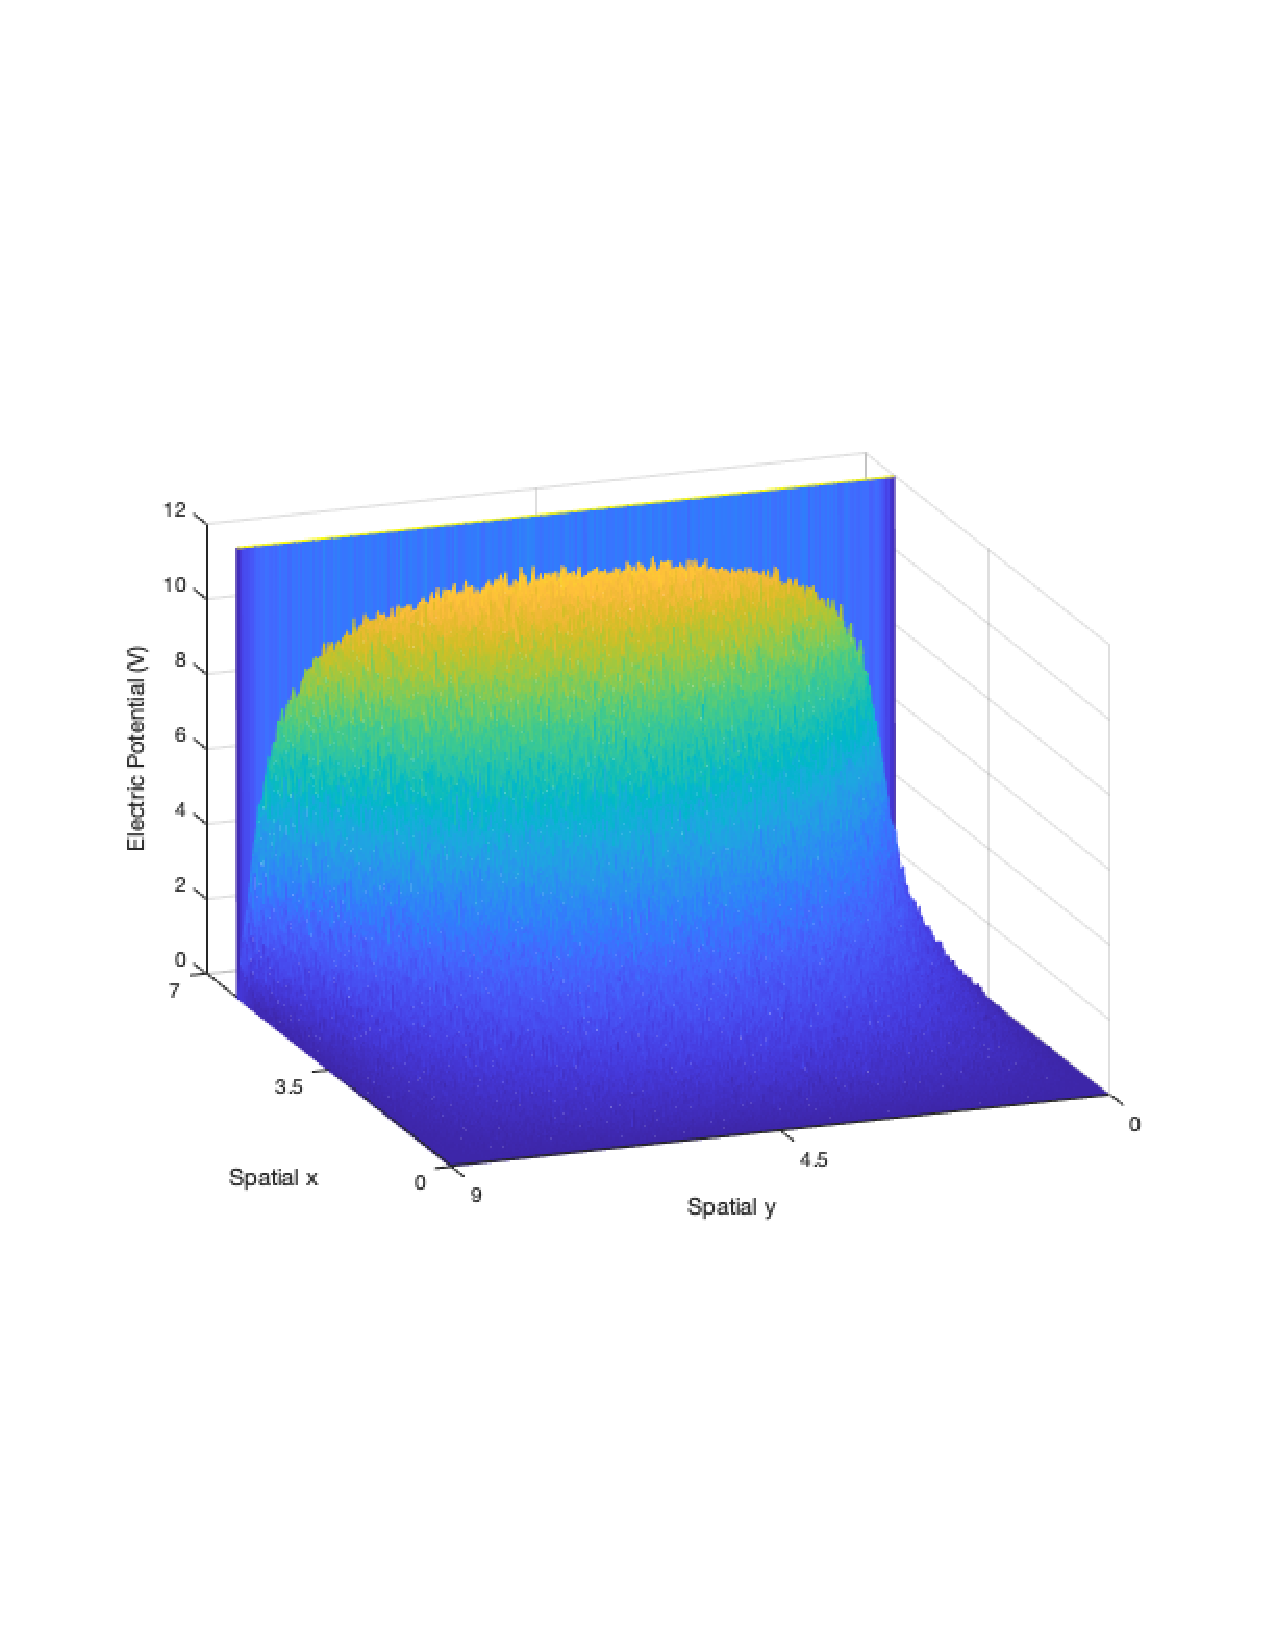
\includegraphics[width=0.48\textwidth]{solution_Dec11_9hrs_isoview.pdf}
	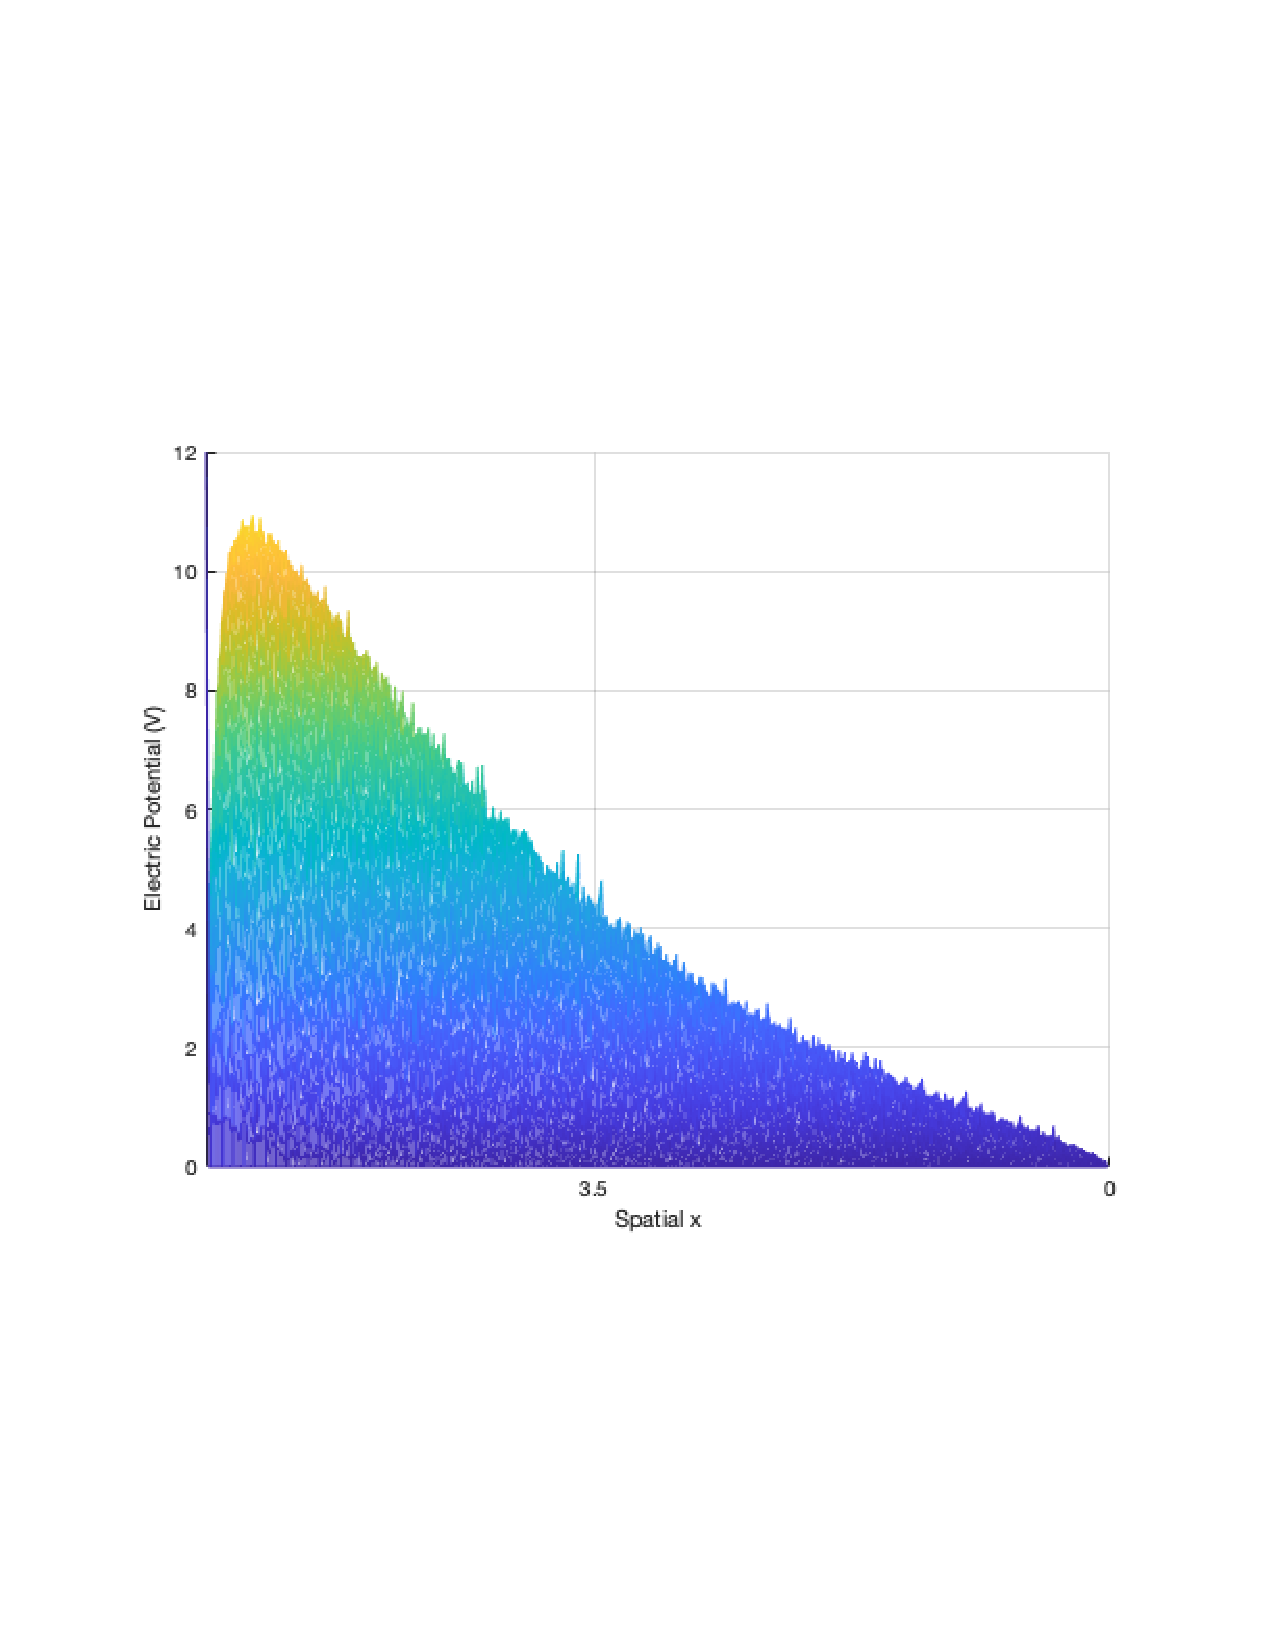
\includegraphics[width=0.48\textwidth]{solution_Dec11_9hrs_sideview.pdf}
\end{figure}

\subsection{Convergence Towards Analytical Solution}

\subsection{Computation Time}

\end{document}